\documentclass[11pt,preprint, authoryear]{elsarticle}

\usepackage{lmodern}
%%%% My spacing
\usepackage{setspace}
\setstretch{1.2}
\DeclareMathSizes{12}{14}{10}{10}

% Wrap around which gives all figures included the [H] command, or places it "here". This can be tedious to code in Rmarkdown.
\usepackage{float}
\let\origfigure\figure
\let\endorigfigure\endfigure
\renewenvironment{figure}[1][2] {
    \expandafter\origfigure\expandafter[H]
} {
    \endorigfigure
}

\let\origtable\table
\let\endorigtable\endtable
\renewenvironment{table}[1][2] {
    \expandafter\origtable\expandafter[H]
} {
    \endorigtable
}


\usepackage{ifxetex,ifluatex}
\usepackage{fixltx2e} % provides \textsubscript
\ifnum 0\ifxetex 1\fi\ifluatex 1\fi=0 % if pdftex
  \usepackage[T1]{fontenc}
  \usepackage[utf8]{inputenc}
\else % if luatex or xelatex
  \ifxetex
    \usepackage{mathspec}
    \usepackage{xltxtra,xunicode}
  \else
    \usepackage{fontspec}
  \fi
  \defaultfontfeatures{Mapping=tex-text,Scale=MatchLowercase}
  \newcommand{\euro}{€}
\fi

\usepackage{amssymb, amsmath, amsthm, amsfonts}

\def\bibsection{\section*{References}} %%% Make "References" appear before bibliography


\usepackage[round]{natbib}

\usepackage{longtable}
\usepackage[margin=2.3cm,bottom=2cm,top=2.5cm, includefoot]{geometry}
\usepackage{fancyhdr}
\usepackage[bottom, hang, flushmargin]{footmisc}
\usepackage{graphicx}
\numberwithin{equation}{section}
\numberwithin{figure}{section}
\numberwithin{table}{section}
\setlength{\parindent}{0cm}
\setlength{\parskip}{1.3ex plus 0.5ex minus 0.3ex}
\usepackage{textcomp}
\renewcommand{\headrulewidth}{0.2pt}
\renewcommand{\footrulewidth}{0.3pt}

\usepackage{array}
\newcolumntype{x}[1]{>{\centering\arraybackslash\hspace{0pt}}p{#1}}

%%%%  Remove the "preprint submitted to" part. Don't worry about this either, it just looks better without it:
\makeatletter
\def\ps@pprintTitle{%
  \let\@oddhead\@empty
  \let\@evenhead\@empty
  \let\@oddfoot\@empty
  \let\@evenfoot\@oddfoot
}
\makeatother

 \def\tightlist{} % This allows for subbullets!

\usepackage{hyperref}
\hypersetup{breaklinks=true,
            bookmarks=true,
            colorlinks=true,
            citecolor=blue,
            urlcolor=blue,
            linkcolor=blue,
            pdfborder={0 0 0}}


% The following packages allow huxtable to work:
\usepackage{siunitx}
\usepackage{multirow}
\usepackage{hhline}
\usepackage{calc}
\usepackage{tabularx}
\usepackage{booktabs}
\usepackage{caption}


\newenvironment{columns}[1][]{}{}

\newenvironment{column}[1]{\begin{minipage}{#1}\ignorespaces}{%
\end{minipage}
\ifhmode\unskip\fi
\aftergroup\useignorespacesandallpars}

\def\useignorespacesandallpars#1\ignorespaces\fi{%
#1\fi\ignorespacesandallpars}

\makeatletter
\def\ignorespacesandallpars{%
  \@ifnextchar\par
    {\expandafter\ignorespacesandallpars\@gobble}%
    {}%
}
\makeatother

\newlength{\cslhangindent}
\setlength{\cslhangindent}{1.5em}
\newenvironment{CSLReferences}%
  {\setlength{\parindent}{0pt}%
  \everypar{\setlength{\hangindent}{\cslhangindent}}\ignorespaces}%
  {\par}


\urlstyle{same}  % don't use monospace font for urls
\setlength{\parindent}{0pt}
\setlength{\parskip}{6pt plus 2pt minus 1pt}
\setlength{\emergencystretch}{3em}  % prevent overfull lines
\setcounter{secnumdepth}{5}

%%% Use protect on footnotes to avoid problems with footnotes in titles
\let\rmarkdownfootnote\footnote%
\def\footnote{\protect\rmarkdownfootnote}
\IfFileExists{upquote.sty}{\usepackage{upquote}}{}

%%% Include extra packages specified by user
\usepackage{booktabs}
\usepackage{longtable}
\usepackage{array}
\usepackage{multirow}
\usepackage{wrapfig}
\usepackage{float}
\usepackage{colortbl}
\usepackage{pdflscape}
\usepackage{tabu}
\usepackage{threeparttable}
\usepackage{threeparttablex}
\usepackage[normalem]{ulem}
\usepackage{makecell}
\usepackage{xcolor}

%%% Hard setting column skips for reports - this ensures greater consistency and control over the length settings in the document.
%% page layout
%% paragraphs
\setlength{\baselineskip}{12pt plus 0pt minus 0pt}
\setlength{\parskip}{12pt plus 0pt minus 0pt}
\setlength{\parindent}{0pt plus 0pt minus 0pt}
%% floats
\setlength{\floatsep}{12pt plus 0 pt minus 0pt}
\setlength{\textfloatsep}{20pt plus 0pt minus 0pt}
\setlength{\intextsep}{14pt plus 0pt minus 0pt}
\setlength{\dbltextfloatsep}{20pt plus 0pt minus 0pt}
\setlength{\dblfloatsep}{14pt plus 0pt minus 0pt}
%% maths
\setlength{\abovedisplayskip}{12pt plus 0pt minus 0pt}
\setlength{\belowdisplayskip}{12pt plus 0pt minus 0pt}
%% lists
\setlength{\topsep}{10pt plus 0pt minus 0pt}
\setlength{\partopsep}{3pt plus 0pt minus 0pt}
\setlength{\itemsep}{5pt plus 0pt minus 0pt}
\setlength{\labelsep}{8mm plus 0mm minus 0mm}
\setlength{\parsep}{\the\parskip}
\setlength{\listparindent}{\the\parindent}
%% verbatim
\setlength{\fboxsep}{5pt plus 0pt minus 0pt}



\begin{document}



\begin{frontmatter}  %

\title{MSCI Funds}

% Set to FALSE if wanting to remove title (for submission)




\author[Add1]{Sven Wellmann}
\ead{20850980@sun.ac.za}





\address[Add1]{Stellenbosch University, Stellenbosch, South Africa}



\vspace{1cm}





\vspace{0.5cm}

\end{frontmatter}



%________________________
% Header and Footers
%%%%%%%%%%%%%%%%%%%%%%%%%%%%%%%%%
\pagestyle{fancy}
\chead{}
\rhead{}
\lfoot{}
\rfoot{\footnotesize Page \thepage}
\lhead{}
%\rfoot{\footnotesize Page \thepage } % "e.g. Page 2"
\cfoot{}

%\setlength\headheight{30pt}
%%%%%%%%%%%%%%%%%%%%%%%%%%%%%%%%%
%________________________

\headsep 35pt % So that header does not go over title




\hypertarget{introduction}{%
\section{\texorpdfstring{Introduction
\label{Introduction}}{Introduction }}\label{introduction}}

This report uses the return profiles of different asset classes to
investigate if diversification ability has decreased in the last decade.
The main methodology will be with the use of a DCC model allowing for
correlations between series to vary over time.

\hypertarget{data}{%
\subsection{Data}\label{data}}

The data I include is the MSCA\_ACWI, EURO\_10Yr, MSCI\_USREIT and the
Oil\_Brent.

\hypertarget{test-the-data}{%
\subsection{Test the data}\label{test-the-data}}

First we will look at the March test which indicates that all the MV
portmanteau tests reject the null of no conditional heteroskedasticity,
motivating the use of MVGARCH models.

\begin{verbatim}
## Q(m) of squared series(LM test):  
## Test statistic:  1.86752  p-value:  0.9972583 
## Rank-based Test:  
## Test statistic:  3732.492  p-value:  0 
## Q_k(m) of squared series:  
## Test statistic:  8118.375  p-value:  0 
## Robust Test(5%) :  3741.885  p-value:  0
\end{verbatim}

\hypertarget{implement-dcc-model}{%
\subsection{Implement DCC Model}\label{implement-dcc-model}}

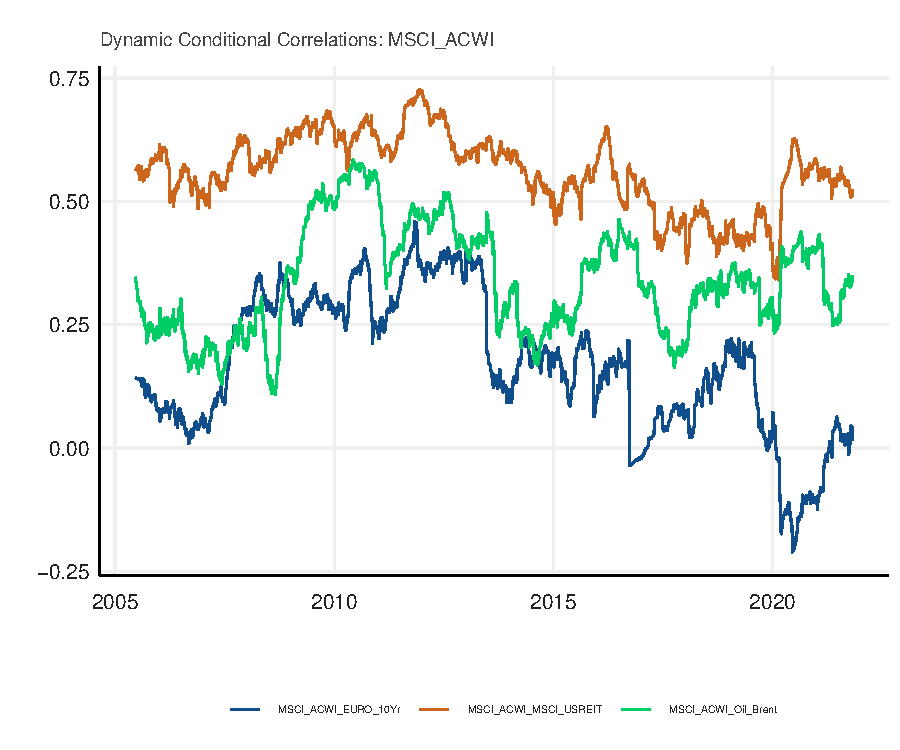
\includegraphics{Question6_files/figure-latex/unnamed-chunk-7-1.pdf}

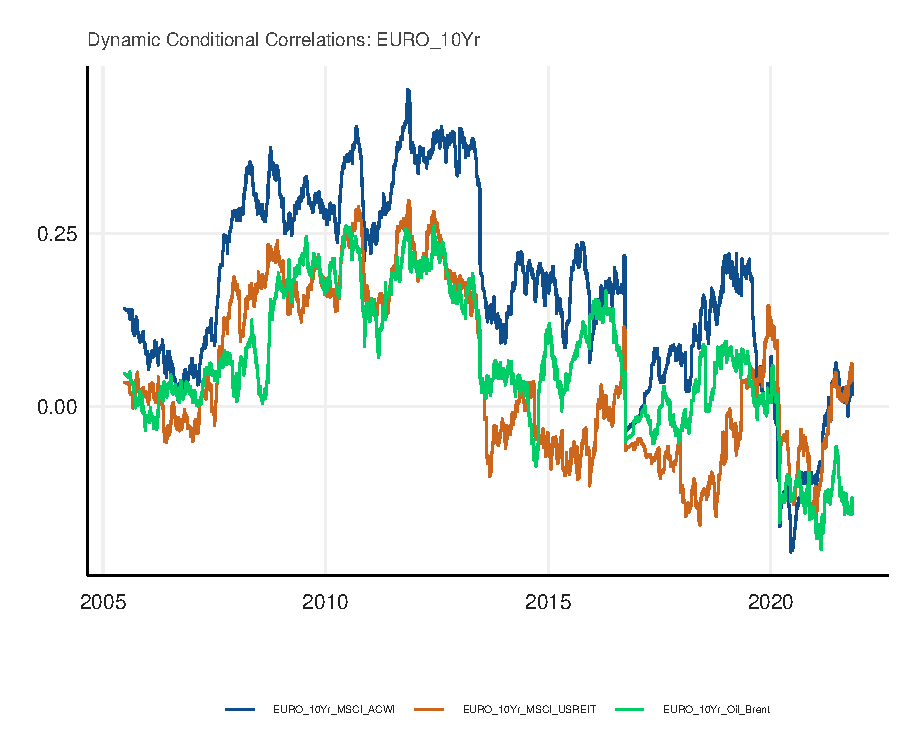
\includegraphics{Question6_files/figure-latex/unnamed-chunk-8-1.pdf}

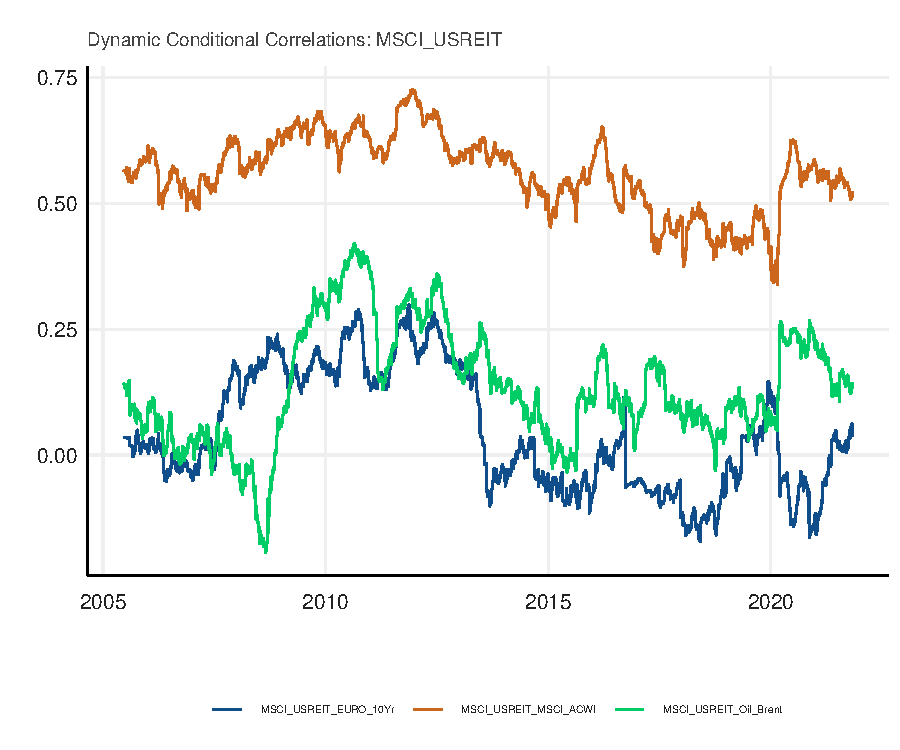
\includegraphics{Question6_files/figure-latex/unnamed-chunk-9-1.pdf}

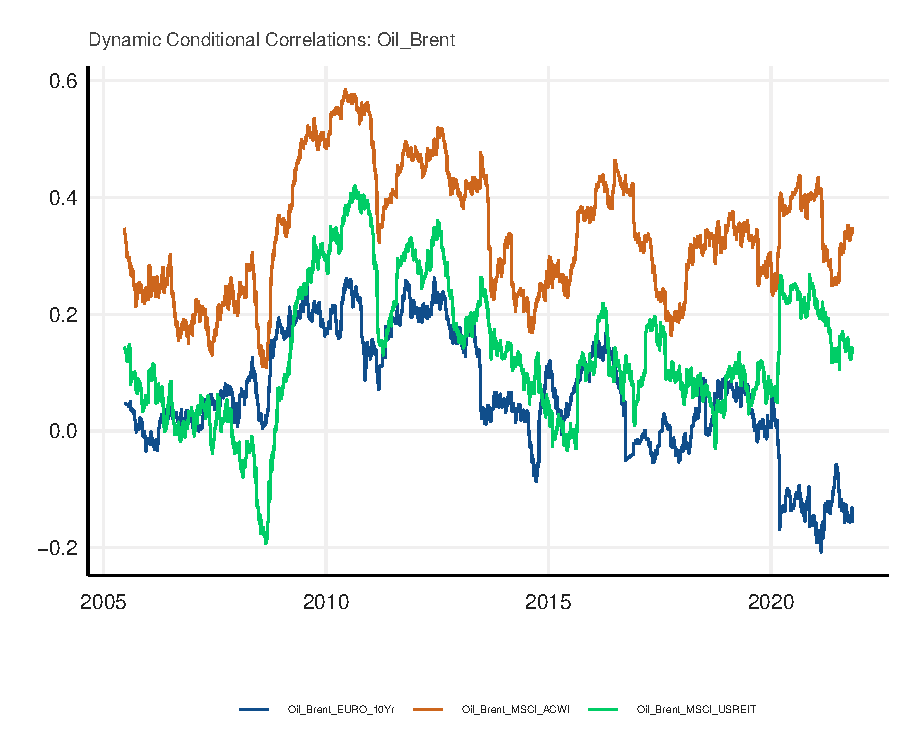
\includegraphics{Question6_files/figure-latex/unnamed-chunk-10-1.pdf}

\begin{verbatim}
## 
## *------------------------------*
## *        GO-GARCH Fit          *
## *------------------------------*
## 
## Mean Model       : CONSTANT
## GARCH Model      : sGARCH
## Distribution : mvnorm
## ICA Method       : fastica
## No. Factors      : 4
## No. Periods      : 4269
## Log-Likelihood   : 46768.8
## ------------------------------------
## 
## U (rotation matrix) : 
## 
##          [,1]     [,2]     [,3]     [,4]
## [1,]  0.99998 -0.00172 -0.00608 -0.00117
## [2,] -0.00239  0.66028 -0.65146  0.37366
## [3,] -0.00195 -0.66138 -0.26866  0.70028
## [4,]  0.00564  0.35581  0.70949  0.60827
## 
## A (mixing matrix) : 
## 
##           [,1]      [,2]    [,3]     [,4]
## [1,]  0.000159 -3.29e-05 0.01021 -0.00114
## [2,] -1.540173  2.64e-03 0.00937  0.00180
## [3,]  0.000227  7.14e-04 0.01093 -0.01676
## [4,]  0.000240 -2.08e-02 0.00939 -0.00028
\end{verbatim}

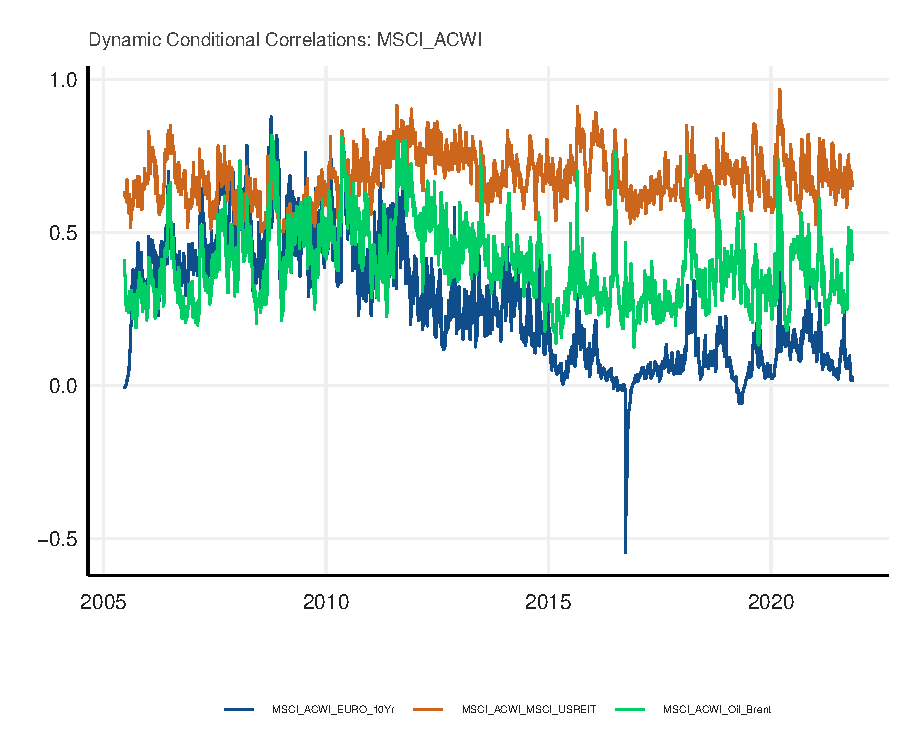
\includegraphics{Question6_files/figure-latex/unnamed-chunk-14-1.pdf}

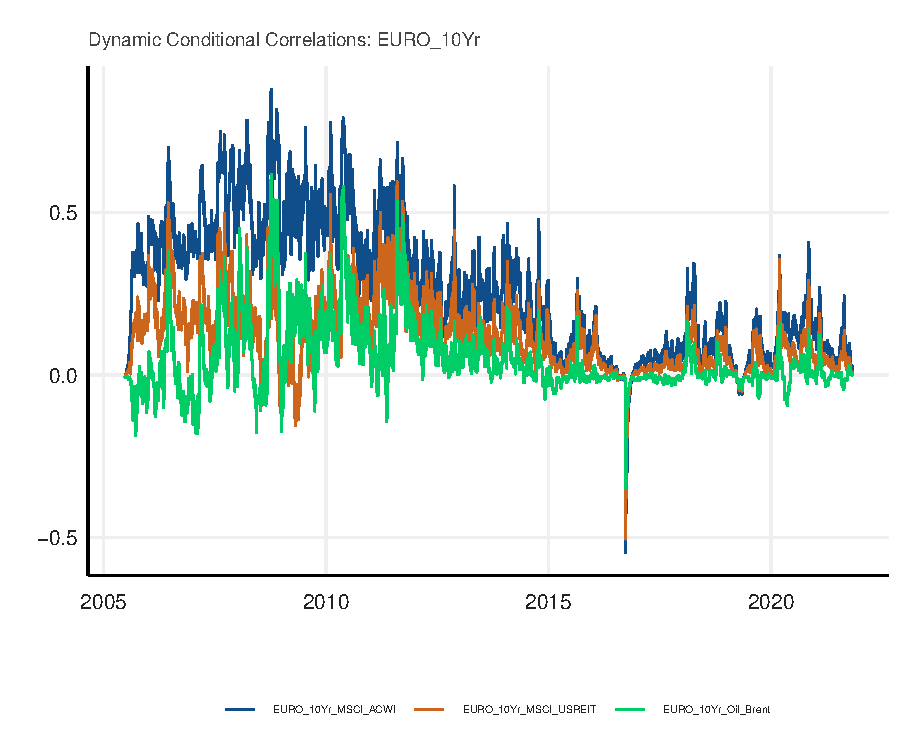
\includegraphics{Question6_files/figure-latex/unnamed-chunk-15-1.pdf}

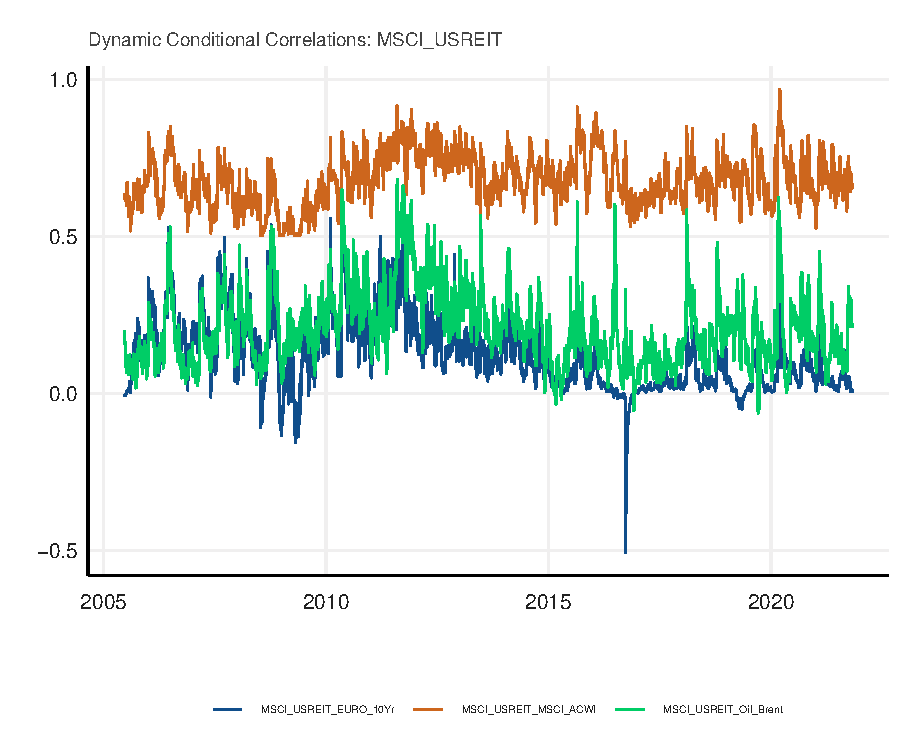
\includegraphics{Question6_files/figure-latex/unnamed-chunk-16-1.pdf}

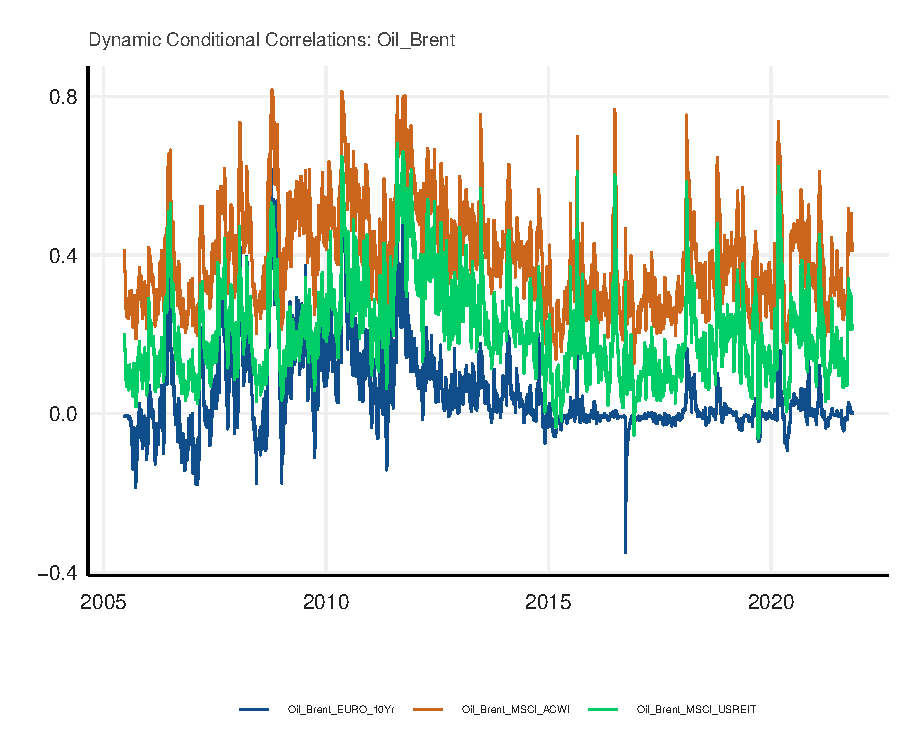
\includegraphics{Question6_files/figure-latex/unnamed-chunk-17-1.pdf}

\hypertarget{conclusion}{%
\section{Conclusion}\label{conclusion}}

\bibliography{Tex/ref}





\end{document}
